% =====================================================================
% Relatório da Entrega 1 -- Engenharia de Usabilidade (UnDF, 2/2026)
% Compilar com: latexmk -pdf (pdfLaTeX) ou -xelatex. Fonte única: Times.
% Todas as páginas em A4 retrato, sem páginas giradas.
% =====================================================================
\documentclass[
  12pt,
  oneside,
  a4paper,
  chapter=TITLE,
  section=TITLE,
  english,
  brazilian
]{abntex2}

\usepackage{iftex}
\ifPDFTeX
  \usepackage[T1]{fontenc}
  \usepackage[utf8]{inputenc}
  \usepackage{mathptmx}
  % Uma única família em todo o documento: Times também no lugar de
  % Helvetica (sf) e Courier (tt).
  \renewcommand{\sfdefault}{ptm}
  \renewcommand{\ttdefault}{ptm}
\else
  \usepackage{fontspec}
  \IfFontExistsTF{Times New Roman}{%
    \setmainfont{Times New Roman}\setsansfont{Times New Roman}\setmonofont{Times New Roman}}{%
    \IfFontExistsTF{Liberation Serif}{%
      \setmainfont{Liberation Serif}\setsansfont{Liberation Serif}\setmonofont{Liberation Serif}}{%
      \setmainfont{TeX Gyre Termes}\setsansfont{TeX Gyre Termes}\setmonofont{TeX Gyre Termes}}}
\fi
\usepackage{indentfirst}
\usepackage{graphicx}
\graphicspath{{./}{../}}
\usepackage{xcolor}
\usepackage{tabularx}
\usepackage{booktabs}
\usepackage{placeins}
\usepackage{microtype}
\usepackage[alf]{abntex2cite}
\usepackage{url}
\urlstyle{same}
\Urlmuskip=0mu plus 1mu
% NBR 6023:2018: endereço eletrônico sem os sinais < >
\def\UrlLeft{}\def\UrlRight{}

\renewcommand{\arraystretch}{1.15}
\newcolumntype{Y}{>{\raggedright\arraybackslash}X}
\newcolumntype{P}[1]{>{\raggedright\arraybackslash}p{#1}}
\setlength{\emergencystretch}{3em}
\raggedbottom
\renewcommand{\topfraction}{0.9}
\renewcommand{\bottomfraction}{0.9}
\renewcommand{\textfraction}{0.08}
\renewcommand{\floatpagefraction}{0.75}
\setcounter{topnumber}{3}
\setcounter{bottomnumber}{3}
\setcounter{totalnumber}{6}
\makeatletter
\setlength{\@fptop}{0pt}
\makeatother
\AtBeginDocument{%
  \renewcommand{\fonte}[1]{\par\vspace{3pt}{\footnotesize\raggedright\noindent Fonte: #1\par}\vspace{4pt}}%
  \renewcommand{\nota}[1]{\par\vspace{2pt}{\footnotesize\raggedright\noindent Nota: #1\par}\vspace{4pt}}%
}

% Quadro como flutuante próprio (mesmo padrão de lista de quadros)
\newcommand{\quadroname}{Quadro}
\newcommand{\listofquadrosname}{Lista de quadros}
\newfloat[chapter]{quadro}{loq}{\quadroname}
\newlistof{listofquadros}{loq}{\listofquadrosname}
\newlistentry{quadro}{loq}{0}
\setfloatadjustment{quadro}{\centering}
\counterwithout{quadro}{chapter}
\renewcommand{\cftquadroname}{\quadroname\space}
\renewcommand*{\cftquadroaftersnum}{\hfill\textendash\hfill}

\newcommand{\preencher}[1]{\textcolor{red}{[#1]}}

% Figura: \fig[largura]{rótulo}{arquivo}{legenda}{fonte}
\newcommand{\fig}[5][0.95]{%
  \begin{figure}[!htbp]
    \centering
    \caption{#4}\label{fig:#2}
    \includegraphics[width=#1\textwidth,height=0.42\textheight,keepaspectratio]{figuras/#3}
    \fonte{#5}
  \end{figure}\FloatBarrier}
\newcommand{\capt}[1]{Secretaria de Economia do DF (#1), acesso em 18 out. 2026}

% Requisitos de usabilidade: uma linha por requisito, agrupados por dimensão
\newcommand{\rudim}{}
\newcommand{\rulinha}[5]{%
  #1\newline\rudim & #2 & #3 & #4 & #5 \\\hline}

% Persona: \persona{n}{título}{perfil e base}{classe}{meta}{recursos}{traços e dificuldades}
\newcommand{\persona}[7]{%
  \begin{quadro}[!htbp]
    \caption{Persona #1 --- #2}\label{qua:persona#1}
    \centering\small
    \begin{tabularx}{\textwidth}{|P{3.1cm}|Y|}\hline
      Perfil e base      & #3 \\\hline
      Classe de contexto & #4 \\\hline
      Meta no serviço    & #5 \\\hline
      Recursos           & #6 \\\hline
      Traços e dificuldades & #7 \\\hline
    \end{tabularx}
    \fonte{Elaborado pelos autores (2026).}
  \end{quadro}}

% ---------------------------------------------------------------------
% Dados do trabalho
% ---------------------------------------------------------------------
\titulo{Solicitação de emissão da guia de ITBI no portal da Secretaria de Economia do DF}
\autor{%
  Ícaro Marra Souza\\
  Karoline Rodrigues Costa\\
  Leonardo Brito Gomes\\
  Luiz Gustavo Silva Carvalho}
\local{Brasília}
\data{out. 2026}
\instituicao{%
  Universidade do Distrito Federal -- UnDF
  \par
  Unidade Curricular de Engenharia de Usabilidade}
\tipotrabalho{Relatório técnico}
\preambulo{Relatório refrente à entrega 1 do projeto da Unidade Curricular de
Engenharia de Usabilidade, apresentado à Universidade do Distrito Federal como
requisito de avaliação, sob orientação da Profa. Dr. Carolina Gonçalves Abreu.}

\definecolor{blue}{RGB}{41,5,195}
\makeatletter
\hypersetup{
  pdftitle={\@title},
  pdfauthor={\@author},
  pdfsubject={UCEngUs -- Entrega 1},
  pdfcreator={LaTeX com abnTeX2},
  pdfkeywords={usabilidade}{acessibilidade}{serviço público digital}{ISO 9241-11},
  colorlinks=true,
  linkcolor=blue,
  citecolor=blue,
  filecolor=magenta,
  urlcolor=blue,
  bookmarksdepth=4}
\makeatother

\renewcommand{\imprimircapa}{%
  \begin{capa}%
    \center
    \IfFileExists{../../assets/marca/undf-vertical.pdf}{%
      \includegraphics[width=4.5cm]{../../assets/marca/undf-vertical.pdf}\par}{%
      \IfFileExists{undf-vertical.pdf}{\includegraphics[width=4.5cm]{undf-vertical.pdf}\par}{%
        \textcolor{red}{[marca UnDF vertical, mínimo 4 cm]}\par}}
    \vspace*{1cm}
    \ABNTEXchapterfont\large\imprimirautor

    \vfill
    \begin{center}
    \ABNTEXchapterfont\bfseries\LARGE\imprimirtitulo
    \end{center}
    \vfill

    \large\imprimirlocal

    \large\imprimirdata

    \vspace*{1cm}
  \end{capa}}

\setlength{\parindent}{1.25cm}
\setlength{\parskip}{0.2cm}

\makeindex

% =====================================================================
\begin{document}
\selectlanguage{brazil}
\frenchspacing

\pretextual

\imprimircapa
\imprimirfolhaderosto

\begin{resumo}
Este relatório mostra o diagnóstico do contexto de uso do trecho do portal da
Secretaria de Economia do Distrito Federal que leva ao formulário de emissão da
guia do Imposto sobre a Transmissão de Bens Imóveis (ITBI) e especifica
requisitos de usabilidade e de acessibilidade para ele. O trecho vai da página
inicial até o formulário de Atendimento Virtual com o assunto ``Emitir Guia de
ITBI -- serviço'' selecionado. A equipe fez cinco sessões com participantes
distintos (observação de uso, entrevista ou as duas), cruzou os relatos com cinco
fontes secundárias e inspecionou as telas com leitor de tela NVDA, teclado,
simulação a 320 px e medição de alvos. No caso, só uma das cinco pessoas chegou ao
formulário sem ajuda, e duas encerraram a tentativa sem concluir. A análise
hierárquica de tarefas auxiliou na indentificação de onde as falhas se concentram, e o diagnóstico
levou a doze pontos observados, muitos deles ligados a um vocabulário interno do órgão e não do
cidadão. Dele foram criadas sete personas, três classes de contexto, oito requisitos de
usabilidade e doze de acessibilidade (WCAG 2.2, nível AA); nenhum dos doze é
atendido hoje. Entre as limitações estão o tamanho da amostra e a ausência de
usuários de leitor de tela entre os participantes.

Palavras-chave: usabilidade, acessibilidade, serviço público digital,
contexto de uso, requisitos.
\end{resumo}

\listoffigures*
\cleardoublepage
\listofquadros*
\cleardoublepage
\listoftables*
\cleardoublepage

\begin{siglas}
  \item[DSGov]  Design System do Governo Federal
  \item[HTA]    \textit{Hierarchical Task Analysis} (Análise Hierárquica de Tarefas)
  \item[IC]     Intervalo de confiança
  \item[ISO]    \textit{International Organization for Standardization}
  \item[ITBI]   Imposto sobre a Transmissão de Bens Imóveis \textit{inter vivos}
  \item[ITCD]   Imposto sobre Transmissão \textit{Causa Mortis} e Doação
  \item[LBI]    Lei Brasileira de Inclusão da Pessoa com Deficiência
  \item[NVDA]   \textit{NonVisual Desktop Access}
  \item[RA]     Requisito de acessibilidade
  \item[RU]     Requisito de usabilidade
  \item[SEEC]   Secretaria de Estado de Economia do Distrito Federal
  \item[SUS]    \textit{System Usability Scale}
  \item[UnDF]   Universidade do Distrito Federal
  \item[WCAG]   \textit{Web Content Accessibility Guidelines}
\end{siglas}

\tableofcontents*
\cleardoublepage

\textual

% =====================================================================
\chapter{Identificação do serviço}\label{cap:identificacao}
% =====================================================================

Este relatório usa os conceitos da ISO 9241-11:2018, o qual cita que usabilidade é a medida em
que usuários específicos alcançam metas específicas, em um contexto de uso
específico, com eficácia, eficiência e satisfação. Por isso cada requisito
adiante está relacionado a uma classe de contexto e a uma tarefa.

O serviço em questão possui a particularidade de não possuir uma única porta de
entrada, dado que o usuário passa pelo portal institucional
(\texttt{economia.df.gov.br}), depois pelo portal da Receita
(\texttt{receita.fazenda.df.gov.br}) e chega ao Atendimento Virtual
(\texttt{atendimentovirtual.fazenda.df.gov.br}), sendo telas com identidades
visuais diferentes (seção~\ref{sec:padr-int}). A solicitação acontece no
terceiro, depois do login, e o relatório trata só do caminho até ele.

\begin{quadro}[!htbp]
  \caption{Identificação do serviço}\label{qua:identificacao}
  \centering\small
  \begin{tabularx}{\textwidth}{|P{3.4cm}|Y|}\hline
    Serviço & Solicitação de emissão da guia de ITBI (transmissão onerosa de imóvel), por Atendimento Virtual. Início: \url{https://www.economia.df.gov.br/}; formulário: \url{https://atendimentovirtual.fazenda.df.gov.br/}. \\\hline
    Órgão responsável & Secretaria de Estado de Economia do Distrito Federal (SEEC), por meio da Receita do Distrito Federal. \\\hline
    Canais & Portal institucional e portal da Receita (carta de serviços); Atendimento Virtual (pessoa física e jurídica); Agência Virtual (Agênci@net); atendimento presencial por agendamento; telefone (S1 relata tentativa sem êxito). \\\hline
    Natureza da demanda & Obrigação tributária, pois o ITBI incide sobre a transmissão onerosa de imóveis, e o comprovante de pagamento da guia é exigido para registrar a transação. \\\hline
  \end{tabularx}
  \fonte{Elaborado pelos autores com base em \citeonline{seec} e nas sessões S1 a S5 (2026).}
\end{quadro}

% =====================================================================
\chapter{Levantamento de dados}\label{cap:levantamento}
% =====================================================================

\section{Métodos}

Foram usados dois métodos, sendo que, na observação de uso, dissemos à pessoa o cenário (``imagine
que você comprou um imóvel e precisa pagar o imposto pelo Governo do DF'') e a
meta (encontrar onde emitir a guia de ITBI), e ela percorreu o fluxo a partir de
\texttt{economia.df.gov.br}, em geral pensando em voz alta. A equipe não deu
instrução nem corrigiu mas registrou ações, falas e pausas. Sempre que
possível, a pessoa usou o próprio aparelho, no caso um computador em S1, S2 e S3, celular em
S4 e notebook em S5. Na entrevista semiestruturada, as perguntas trataram de uso
anterior, aparelho e lugar, o que deu certo ou errado, busca por ajuda e
comparação com outros serviços do governo (roteiro no
Apêndice~\ref{ap:roteiro}). S1, S2 e S4 combinaram observação e entrevista; S3 foi
só entrevista; S5 foi só observação, registrada em uma nota (Apêndice~\ref{ap:material}).

\section{Sessões}

\begin{table}[!htbp]
  \caption{Sessões de levantamento e perfil dos participantes}\label{tab:sessoes}
  \centering\footnotesize
  \begin{tabularx}{\textwidth}{|P{1.3cm}|P{1.8cm}|P{2.3cm}|Y|P{2.0cm}|P{1.5cm}|}\hline
    Sessão & Data & Método & Perfil (sem nome) & Aparelho & Tempo \\\hline
    S1 (P01) & 05/10/2026 & Observação e entrevista & Mulher, cerca de 40 anos; superior completo; já lidou com ITBI & Computador, em casa & 10 min \\\hline
    S2 (P02) & 06/10/2026 & Observação e entrevista & Mulher, entre 20 e 30 anos; superior completo; habituada à web & Computador de mesa & 9 min \\\hline
    S3 (P03) & 07/10/2026 & Entrevista & Homem idoso; ensino médio completo; já lidou com a questão; depende da esposa para a internet & Computador, em casa & 7 min \\\hline
    S4 (P04) & 08/10/2026 & Observação e entrevista & Mulher, 19 anos (maior de idade); cursando superior; já lidou com compra de imóvel & Celular, em casa & 10 min \\\hline
    S5 (P05) & 19/10/2026 & Observação (nota de campo) & Homem, 23 anos; superior incompleto & Notebook & 19 min 37 s \\\hline
  \end{tabularx}
  \fonte{Elaborada pelos autores (2026).}
  \nota{O código P01 a P05 identifica o participante no Apêndice~\ref{ap:material}. Os tempos de S1 a S4 são totais de sessão.}
\end{table}

\section{Fontes e inspeção própria}\label{sec:fontes}

Fonte primária: as cinco sessões, com suas notas e transcrições
(Apêndices~\ref{ap:consentimento} e~\ref{ap:material}).

Fontes secundárias: TIC Domicílios \cite{ticdomicilios}, para o
dispositivo de acesso à internet; Censo 2022 do IBGE \cite{ibgecenso2022}, para a
relação entre idade e alfabetização; Inaf 2024 \cite{inaf2024}, para alfabetismo
funcional de adultos; levantamento da WebAIM com usuários de leitor de tela
\cite{webaim2024}; e Padrão Digital de Governo \cite{dsgov}.

Inspeção própria: análise das telas do fluxo com Norman
\cite{norman2013}, Gestalt, Fitts \cite{fitts1954} e Hick \cite{hick1952}; medição das razões de contraste nas capturas, com a fórmula da WCAG 2.2
\cite{wcag22}; NVDA e navegação por teclado em quatro endereços do fluxo
(portal institucional, catálogo de ITBI da Receita, tela de cartões do
Atendimento Virtual e formulário); simulação de refluxo no modo responsivo do
navegador, com \textit{viewport} de 320 px, equivalente a zoom de 400\% em uma
janela de 1280 px; medição manual da largura e da altura dos alvos no
inspetor de elementos. A parte do leitor de tela foi feita por um integrante sem deficiência
visual e vale, pois, apenas como uma simulação.

\section{Resultados}

O ITBI se paga uma vez, que é na compra do imóvel, e por isso nenhum dos cinco
participantes usa o serviço com frequência. S1, S3 e S4 já tinham lidado com
ele, e S4 relatou uma compra. S5 parou a busca para perguntar o que é ITBI, o que é um sinal
de que a sigla não é conhecida nem entre pessoas escolarizadas. Três
participantes chegaram ao site por meio de um o atendimento presencial ou terceiros que os orientaram. S3 ouviu que ``agora é tudo por lá e não adiantava ir
pessoalmente''; S1 foi à Secretaria depois de falhar ao telefone, e
``explicaram o que deveria ser feito, como deveria ser feito, que era no site'';
S4 recebeu ``um papelzinho'' com o fluxo. O atendimento presencial age, assim,
como \textit{fallback} que orienta a pessoa a usar o canal digital.

Quanto aos recursos, estão computador (S1, S2, S3), notebook (S5) e celular (S4).
Nenhum dos usuários relatou uma conexão instável, o que não prova que ela não exista, e ninguém
se declarou usuário de tecnologia assistiva.

O Quadro~\ref{qua:sessoes-res} resume as sessões, e o
capítulo~\ref{cap:hta} as localiza na HTA. E o padrão que se encontra é que a pessoa procura
``serviços'' ou ``imposto'' no menu, chega ao catálogo da Receita, não vê
``emitir guia'' em nenhum rótulo e erra por itens vizinhos (S2: lançamento,
cancelamento, segunda via, quitação; S4: ``o lugar onde tinha ITBI'' e depois
``duas abas com o mesmo nome''). Apenas S1 chegou ao formulário, e por um caminho
diferente do previsto na HTA, pois usou o link dentro do texto da página do serviço, e não
o botão ``Atendimento Virtual'' do topo. S5 chegou à tela do Atendimento Virtual
e saiu em poucos segundos sem reconhecê-la.

\begin{quadro}[!htbp]
  \caption{Resultado de cada sessão}\label{qua:sessoes-res}
  \centering\footnotesize
  \begin{tabularx}{\textwidth}{|P{1.2cm}|P{2.6cm}|Y|Y|}\hline
    Sessão & Desfecho & Erros de rota e hesitações & Ajuda ou desistência \\\hline
    S1 & Chegou ao formulário, sem ajuda na sessão & Procurou ``Central de Atendimento ao Cidadão'', rolou sem achar, voltou e reabriu o menu; ``tive que entrar e sair'' & Em tentativas anteriores, ajuda de familiares e de servidores \\\hline
    S2 & Não localizou; encerrou após explorar itens errados do catálogo & Percorreu lançamento, cancelamento, segunda via e quitação; ``não sei, não estou achando'' & Encerrou sem concluir \\\hline
    S3 & Não chegou & ``Fiquei perdido'', ``tem muita informação espalhada'' & Chamou a esposa; relata cerca de 20 minutos na tentativa \\\hline
    S4 & Não chegou & Clicou em ``ITBI'' no catálogo, viu que não era o lugar, confundiu duas abas com o mesmo nome & Relata IA, familiar e atendente; na sessão, não concluiu \\\hline
    S5 & Não localizou; desistiu & Ao menos cinco buscas sem chegar ao formulário; manual em PDF e \textit{Ctrl+F}; requerimentos baixados; Google; três sites alternados; visitou o Atendimento Virtual e saiu sem reconhecê-lo & Desistiu aos 19 min 37 s; reclamou dos sites do governo \\\hline
  \end{tabularx}
  \fonte{Elaborado pelos autores com base em S1 a S5 (2026).}
\end{quadro}\FloatBarrier

Quanto às classes de contexto, foram identificados 4 contrastes, sendo o de familiaridade, sendo que S1, S2 e S5 se mostram habituados
à web, e mesmo assim S2 e S5 não
chegaram ao formulário e S1 precisou ser ``muito analítica''; saber usar a web não
protege contra o problema, já S3 e S4 pediram ajuda. O
segundo é a percepção do texto, pois S1 achou os tamanhos de texto e de botão
``bons'', enquanto S3 disse que ``as letras às vezes são pequenas''. A divergência
mostra que a legibilidade depende de idade e aparelho e não tem como solução um
tamanho único. O terceiro é a estratégia de recuperação, pois S1 se recuperou
sozinha por navegação lateral, S5 recorreu a fontes externas, S3 e S4 chamaram
terceiros, e S2 supôs que ``uma senhora de 60 anos'' não conseguiria. E o quarto é o aparelho, dado que S4, no celular, descreve ``muita
informação'' e ``um monte de botão''.

% =====================================================================
\chapter{Contexto de uso}\label{cap:contexto}
% =====================================================================

\section{Usuários}

Quanto a quem utiliza a ferramente em questão, está qualquer pessoa física que compre um imóvel no Distrito Federal, de vinte a
oitenta anos, com qualquer escolaridade e qualquer familiaridade com a web. A frequência de uso é baixa, sendo um evento por
transação imobiliária. Há
também usuários indiretos que a amostra não cobre, como corretores, despachantes
e contadores.

\section{Metas e tarefas}

A meta maior é, sobretudo, concluir a compra de um imóvel. No serviço, a meta é obter a
guia de ITBI, o que exige achar o caminho no portal, chegar ao
Atendimento Virtual, autenticar-se, preencher o formulário e emitir a guia. Este
relatório trata só de encontrar e abrir o formulário, trecho em que as sessões
registraram as falhas. Então, o peso de não concluir custa o adiamento da transação, uma ida a um
posto de atendimento (S1) e a dependência de outra pessoa (S1, S3, S4).

\section{Recursos}\label{sec:recursos}

Dado que o celular é o dispositivo predominante de acesso à internet no país
\cite{ticdomicilios}, interssante observar que S4 diz usar ``geralmente celular'' para sites de governo.
Além do mias, os documentos exigidos
são desconhecidos previamente e o portal não os mostra antes do login (A8). O
Atendimento Virtual pede CPF e senha e oferece ``Cadastre-se''; criar a conta
está fora do escopo, mas mesmo assim é um bloqueio a mais. E, por fim, o apoio vem de familiares,
servidores da Secretaria e, em S4, de uma ferramenta de IA.

\section{Ambiente}

No quesito técnico, são três subdomínios (apesar de ser um serviço, são sites diferentes) com cabeçalhos, menus e identidade
visual diferentes (Figura~\ref{fig:achado2}), um menu \textit{dropdown} de dois
níveis no portal e um catálogo de três colunas na Receita. A partir das
sessões, o local de uso informado pelos usuários foi que que acessam por casa. Além disso, a pessoa costuma ser mandada ao site por um atendente ou conhecido
e pode ter ao lado alguém com ``mais paciência'' (S3). Já no sentido organizacional,
atendimento presencial, telefone e site são as opções, e o
roteiro impresso que S4 recebeu expressa que o
caminho no site não é suficiente sozinho.

% =====================================================================
\chapter{Fluxo crítico}\label{cap:fluxo}
% =====================================================================

\section{Delimitação}

\begin{quadro}[!htbp]
  \caption{Delimitação}\label{qua:fluxo}
  \centering\small
  \begin{tabularx}{\textwidth}{|P{3.4cm}|Y|}\hline
    Fluxo & Encontrar e abrir, a partir da página inicial da Secretaria de Economia do DF, o formulário de Atendimento Virtual para solicitar a emissão da guia de ITBI. \\\hline
    Início & Página inicial \texttt{economia.df.gov.br}, sem login (cenário de S1, S2, S4 e S5). Entradas por busca externa ou por link recebido não foram avaliadas. \\\hline
    Término & Formulário ``Atendimento Virtual -- Registrar solicitação'' exibido, com Assunto = ITBI (marca verde) e o campo ``Tipo de Atendimento'' ainda em ``Selecione'' (Figura~\ref{fig:fluxo-form}). \\\hline
    Fora do escopo & Criação de conta e login; escolha do tipo de atendimento e preenchimento do formulário; emissão e pagamento da guia; etapas presenciais; outros serviços de ITBI do catálogo (cancelamento, impugnação, restituição, quitação, isenção). \\\hline
  \end{tabularx}
  \fonte{Elaborado pelos autores (2026).}
\end{quadro}

As cinco telas do caminho (Figuras~\ref{fig:fluxo-home} a~\ref{fig:fluxo-form})
formam a evidência das análises feitas.

\fig[0.78]{fluxo-home}{fig_home.png}{Tela 1: portal institucional com o menu Serviços aberto (\texttt{economia.df.gov.br})}{\capt{\texttt{economia.df.gov.br}}.}
\fig[0.78]{fluxo-cat}{fig_cat.png}{Tela 2: portal da Receita, ``Para o Cidadão'', com o catálogo aberto em ITBI (\texttt{receita.fazenda.df.gov.br})}{\capt{\texttt{receita.fazenda.df.gov.br}}.}
\fig[0.78]{fluxo-serv}{fig_serv.png}{Tela 3: página de um serviço do catálogo}{\capt{\texttt{receita.fazenda.df.gov.br}}.}
\fig[0.78]{fluxo-atv}{fig_atv.png}{Tela 4: Atendimento Virtual (\texttt{atendimentovirtual.fazenda.df.gov.br})}{\capt{\texttt{atendimentovirtual.fazenda.df.gov.br}}.}
\fig[0.78]{fluxo-form}{fig_form.png}{Tela 5: formulário de registro de solicitação com Assunto = ITBI }{\capt{\texttt{atendimentovirtual.fazenda.df.gov.br}}.}

\section{Justificativa}

A guia é um pré-requisito de uma transação de alto
valor e o serviço não tem uma alternativa equivalente, já que o atendimento presencial
pede a pessoa que acesse o site. O que revela a extrema importancia do usuário conseguir ter sucesso na emissão.
Além do mais, nas cinco sessões as pessoas relataram ou demonstaram
dificuldade, sendo que quatro de cinco não chegaram ao formulário
(Quadro~\ref{qua:sessoes-res}).

% =====================================================================
\chapter{Personas}\label{cap:personas}
% =====================================================================

Seguimos \citeonline{cooper1999} e baseamos as personas nos dados provenientes das entervistas com os usuários. Assim, as
personas 1, 2, 3 e 7 têm base primária (S1 a S5) e as personas 4, 5 e 6 têm base
secundária. Vale ressaltar que os nomes abaixo são fictícios.

\persona{1}{Antônio, pessoa idosa}%
  {Perfil: pessoa idosa. Base primária: S3 (entrevista).}%
  {C2: eventual com baixo letramento digital, dependente de apoio.}%
  {Emitir a guia pelo site, porque lhe disseram que ``agora é tudo por lá''.}%
  {Computador em casa; ensino médio completo; sem conta nem lista de documentos; cerca de 20 minutos para tentar.}%
  {Entrou ``direto no site da Secretaria'' e procurou ``a parte de imposto''; ficou perdido com ``esse tanto de botão'', letras pequenas e informação escondida; desistiu após cerca de 20 minutos e chamou por ajuda. Quer ``os objetivos mais no início da tela''. Dificuldades: excesso de opções, texto pequeno, rótulos que não nomeiam a tarefa.}

\persona{2}{Júlia, 19 anos, usuária de celular}%
  {Perfil: mobile-first (acesso restrito pela tela). Base primária: S4 (entrevista e observação).}%
  {C3: acesso ou percepção restrita (tela pequena).}%
  {Pagar o imposto de um imóvel comprado; já lidou com compra, venda ou recebimento de imóveis.}%
  {Celular, em casa; cursando ensino superior; usa ``geralmente celular''; roteiro em papel do atendimento; apoio de familiares, do atendente e de uma IA.}%
  {Recebeu um detalhamento do fluxo, tentou uma IA, pediu ajuda a familiares e ao atendente; clicou no ``ITBI'' do catálogo e viu que ``não era aquele lugar'', diante de ``duas abas diferentes com o mesmo nome''; não sabia os documentos; não emitiu a guia e ficou ``frustrada e decepcionada''. Dificuldades: homonímia de ITBI, excesso de informação, falta de lista de documentos, refluxo e alvos pequenos (A12, medidos por inspeção, sem teste com usuária real).}

\persona{3}{Camila, familiarizada com a web}%
  {Perfil: usuária familiarizada. Base primária: S1 (observação e entrevista); S2 corrobora.}%
  {C1: familiarizada com a web.}%
  {Encontrar onde emitir a guia de ITBI de um imóvel comprado.}%
  {Computador; ensino superior completo; usa menus e links com desenvoltura; conta com familiares e servidores quando trava.}%
  {Pensa em ``serviços'' ao abrir o site; procurou ``Central de Atendimento ao Cidadão'', rolou, nada, voltou; ``tive que entrar e sair'' e ``ser muito analítica''; chegou por um link no texto do serviço; na vez anterior ligou, não conseguiu e foi ao local; achou texto e botões ``bons'', mas cores ``muito opacas''. Dificuldades: menu que não nomeia a tarefa, itens de natureza diferente com a mesma aparência, nenhum aviso prévio de login.}

\persona{4}{Rosimeire, baixa escolaridade}%
  {Perfil: baixa escolaridade. Base secundária: Censo 2022 \cite{ibgecenso2022} e Inaf 2024 \cite{inaf2024}, com indícios em S3 e S4.}%
  {C2: eventual com baixo letramento digital.}%
  {Obter a guia sem depender de leitura longa; precisa que o rótulo diga o que acontece ao clicar.}%
  {Celular ou computador de uso compartilhado; precisa de ajuda com siglas e termos jurídicos; apoio de terceiros.}%
  {Lê devagar textos longos e estranha termos como ``Transmissão Onerosa'', ``Lançamento'' e ``Impugnação''; precisa reconhecer o que o rótulo faz, não lembrar o que ele é. Dificuldades: siglas sem expansão (ITBI, ITCD), vocabulário jurídico, formulário longo com editor de texto.}

\persona{5}{Valdir, usuário de leitor de tela}%
  {Perfil: leitor de tela. Base secundária: WebAIM \cite{webaim2024}. A inspeção com NVDA confirmou as barreiras técnicas; falta o teste com usuário real.}%
  {C3: acesso ou percepção restrita.}%
  {Chegar ao formulário com leitor de tela e teclado.}%
  {Computador com leitor de tela; navegação por teclado; segundo a WebAIM, a navegação por títulos e regiões é a estratégia usual para localizar informação.}%
  {Depende de títulos, \textit{landmarks} e rótulos de campo. O menu que só abre com o mouse e os cartões sem foco não são alcançáveis por teclado, os ícones sem rótulo do editor (Figura~\ref{fig:achado9}) são lidos como ``Botão'' e o foco fica preso no editor (A11). O efeito real sobre a pessoa depende de teste com usuário. Dificuldades: \textit{dropdown}, catálogo em colunas, editor rico, cartões em imagem (A6).}

\persona{6}{Edilene, acesso precário}%
  {Perfil: acesso precário. Base secundária: TIC Domicílios \cite{ticdomicilios}.}%
  {C3: acesso ou percepção restrita.}%
  {Obter a guia pelo celular com conexão móvel limitada, sem voltar a um posto presencial.}%
  {Celular de entrada, conexão com franquia limitada ou instável, tela pequena; sem computador.}%
  {Cada recarga de página custa tempo, e o fluxo atual exige quatro carregamentos; páginas pesadas abrem devagar, e ela desiste se uma não carrega. A medição de alvos menores que 24 por 24 px (A12) reforça a dificuldade em tela pequena.}

\persona{7}{Rafael, 23 anos, recorre a fontes externas}%
  {Perfil: usuário familiarizado. Base primária: S5 (nota de campo cronometrada).}%
  {C1: familiarizado com a web.}%
  {Encontrar o formulário de emissão da guia de ITBI.}%
  {Notebook; ensino superior incompleto; disposto a gastar quase 20 minutos; usa Google, manuais em PDF e \textit{Ctrl+F}.}%
  {A busca é o primeiro reflexo e, como não funciona, pergunta se ``a barra de pesquisa não funciona?''; pergunta o que é ITBI; chega à Receita por Serviços, Serviços da Receita e Para o Cidadão porque ``preciso de um serviço e sou cidadão''; segue até um manual em PDF, baixa requerimentos, recorre ao Google, visita o Atendimento Virtual e sai sem reconhecê-lo. Dificuldades: busca que devolve documentos e não o formulário, sigla desconhecida, rota correta não reconhecida mesmo quando exibida.}

\begin{quadro}[!htbp]
  \caption{Cobertura dos perfis obrigatórios pelas personas}\label{qua:cobertura}
  \centering\small
  \begin{tabularx}{\textwidth}{|P{4.6cm}|P{1.8cm}|Y|}\hline
    Perfil exigido & Persona & Base \\\hline
    Pessoa idosa & 1 & Primária (S3) \\\hline
    Baixa escolaridade & 4 & Secundária, com indício em S3 e S4 \\\hline
    Usuário de leitor de tela & 5 & Secundária; teste com usuário pendente \\\hline
    Acesso precário & 6 & Secundária \\\hline
    Complementares: celular, familiarizada, busca externa & 2, 3 e 7 & Primária (S4; S1 e S2; S5) \\\hline
  \end{tabularx}
  \fonte{Elaborado pelos autores (2026).}
\end{quadro}

% =====================================================================
\chapter{Análise hierárquica de tarefas}\label{cap:hta}
% =====================================================================

A HTA decompõe o fluxo do capítulo~\ref{cap:fluxo} em objetivo geral, subtarefas
e planos de execução, na linha de \citeonline{annett1967} e
\citeonline{stanton2005}. O objetivo é, assim, acessar o formulário de emissão da guia
a partir de \texttt{economia.df.gov.br}. Ele se divide em três etapas, a primeira
(acessar o site da Secretaria) foi aberta em três subtarefas, por exigir navegação
em menus, e a segunda e a terceira são cliques únicos. Seguindo sem erro, o caminho
previsto tem cinco cliques em quatro carregamentos de página; o caminho de S1,
pelo catálogo, requer sete cliques. A Figura~\ref{fig:hta} marca, com a sessão de
origem, onde houve hesitação (H), erro de rota (E) e abandono ou pedido de ajuda
(A).

\begin{figure}[!htbp]
  \centering
  \caption{Diagrama da HTA do fluxo crítico, com pontos de falha por sessão}\label{fig:hta}
  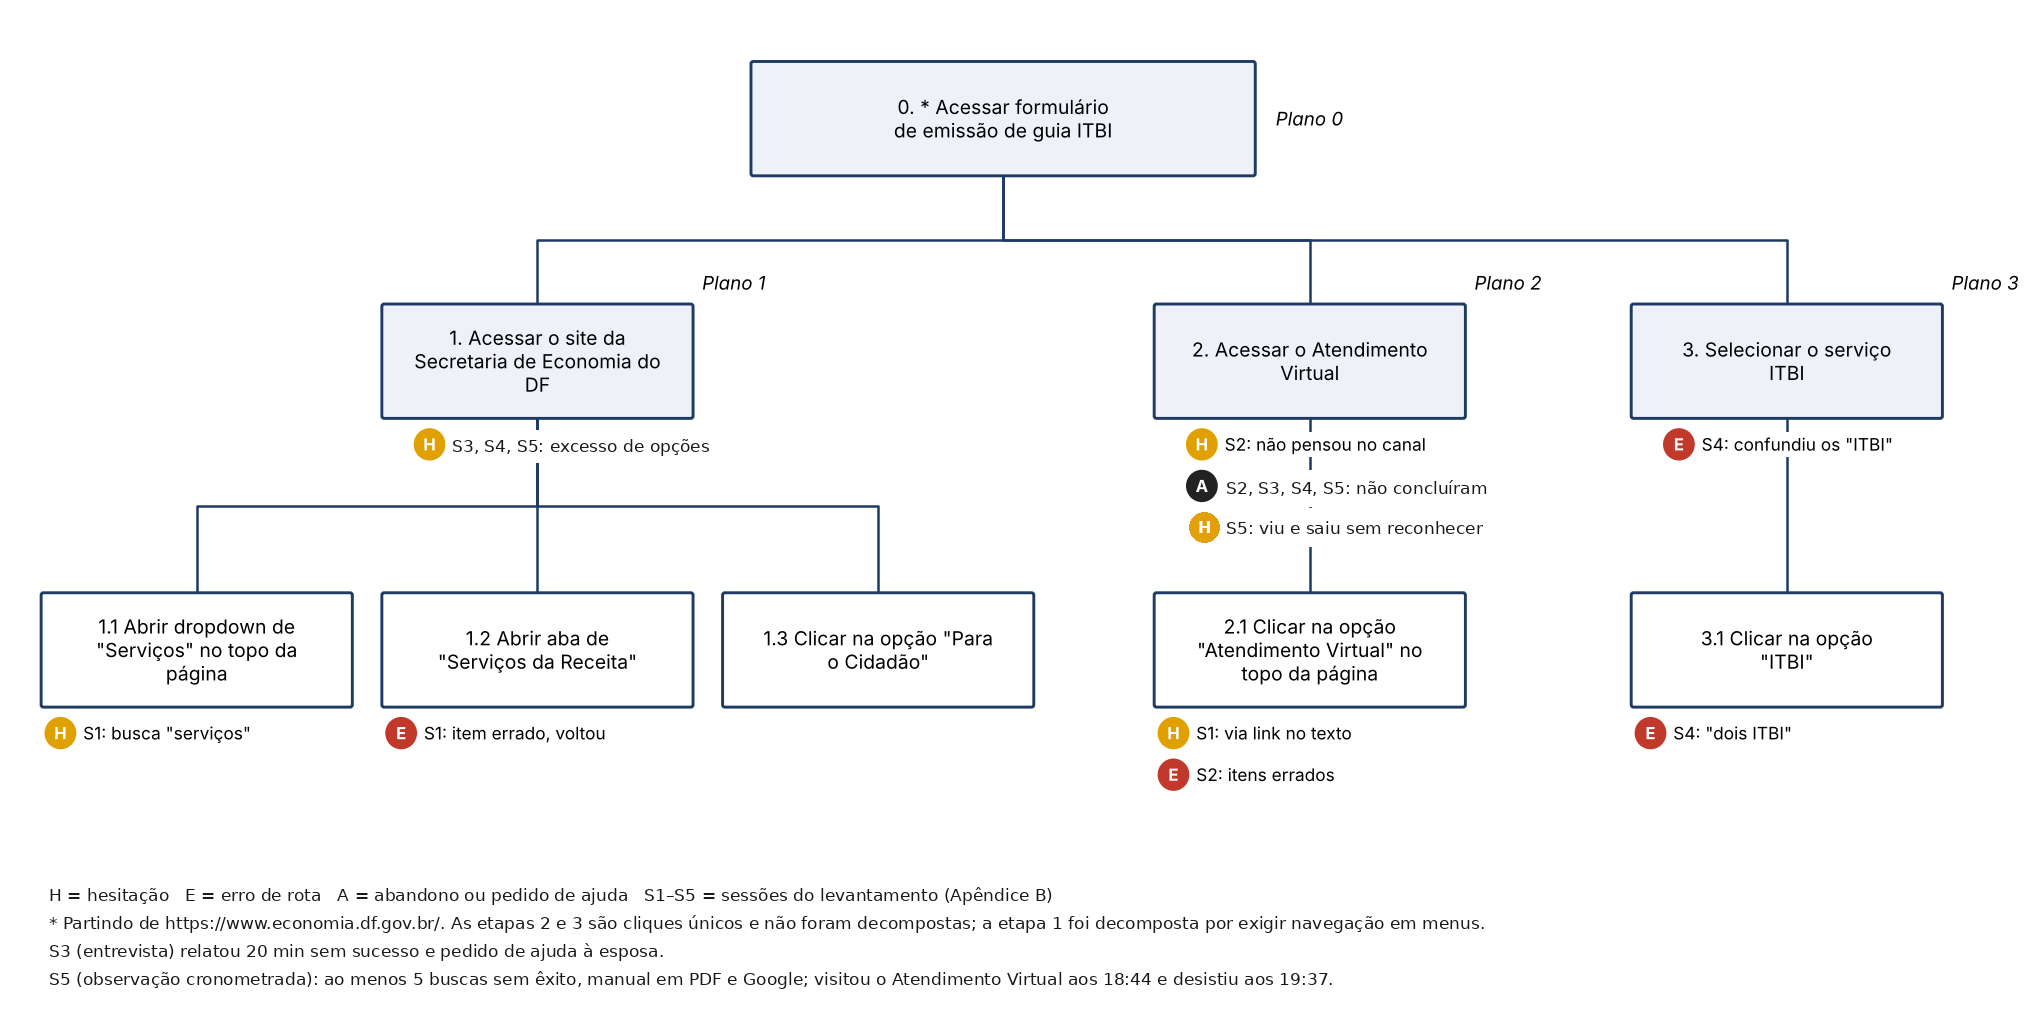
\includegraphics[width=0.95\textwidth,height=0.55\textheight,keepaspectratio]{figuras/hta.png}
  \fonte{Elaborada pelos autores com base em S1 a S5 (2026).}
\end{figure}

\begin{quadro}[!htbp]
  \caption{Planos de execução da HTA}\label{qua:planos}
  \centering\footnotesize
  \begin{tabularx}{\textwidth}{|P{1.3cm}|Y|Y|}\hline
    Plano & Regra de execução & Falhas observadas \\\hline
    0 & Fazer 1, depois 2, depois 3. Encerrar quando o formulário for exibido. & Abandono ou pedido de ajuda na etapa 2: S2, S3, S4 e S5 não chegaram ao formulário. \\\hline
    1 & Fazer 1.1, 1.2 e 1.3. Encerrar quando a página ``Para o Cidadão'' da Receita for exibida, com a faixa de botões (Serviços On-line, Agênci@net, Atendimento Virtual, Legislação) e o catálogo. & Hesitação em 1.1 (S1 procura ``serviços'' e escolhe o item errado); erro de rota em 1.2 (S1 volta e reabre); excesso de opções na etapa (S3, S4, S5; S5 recorreu à busca e ao Google). \\\hline
    2 & Fazer 2.1 (botão ``Atendimento Virtual'' no topo da página da Receita). Variante de S1 (2.1'): do catálogo, abrir ITBI, depois ``Transmissão Onerosa -- Lançamento de ITBI'' e usar o link para o Atendimento Virtual no texto do serviço. & Hesitação em 2 (S2 não pensou no canal ``Atendimento Virtual''); erro de rota em 2.1 (S2: itens errados do catálogo); S5 visitou o Atendimento Virtual e saiu sem reconhecê-lo; S1 só chegou pela variante 2.1'. \\\hline
    3 & Fazer 3.1 (cartão ITBI, em Pessoa Física). & Erro de rota (S4 confundiu o ``ITBI'' do catálogo com o do Atendimento Virtual). \\\hline
  \end{tabularx}
  \fonte{Elaborado pelos autores (2026).}
\end{quadro}

A etapa que concentra as falhas é a 2, não a 1. Quatro das cinco pessoas
navegaram os menus e ainda assim não chegaram ao Atendimento Virtual, ou, em S5,
chegaram e o deixaram sem reconhecê-lo, porque o botão que levaria até lá nomeia
um canal e elas procuravam uma tarefa. Além disso, a única pessoa que concluiu o
fez por um caminho que a HTA original não previa, o que mostra dois
caminhos para o mesmo estado e que o de topo, pensado como principal, não foi o
usado. Como o caminho previsto é curto, a distância entre cinco cliques e a taxa
de falha indica um problema de descoberta e de vocabulário.

% =====================================================================
\chapter{Diagnóstico}\label{cap:diagnostico}
% =====================================================================

O diagnóstico reúne doze achados (A1 a A12) sobre o fluxo delimitado no capítulo~\ref{cap:fluxo}. Eles vêm da inspeção heurística das cinco telas e, quando há dado, da observação de uso das pessoas nas sessões S1 a S5. Os Quadros~\ref{qua:achados1} a~\ref{qua:achados3}, ao fim do capítulo, resumem, para cada achado, a evidência, a origem, os princípios violados e o impacto nas personas.

A1. O menu Serviços lista categorias administrativas, e não tarefas. O menu abre à esquerda com Serviços da Receita, Reforma Tributária, Atendimento, Sistemas, Serviços de TIC, Carta de Serviços, Ouvidoria e Escola de Governo e, no segundo nível, Para o Cidadão, Para o Empresário, Outros Contribuintes, Governo e Parceiros e Agendar Atendimento Presencial (Figura~\ref{fig:achado1}). Ninguém que procura ``emitir guia'' encontra essas palavras, e o item ``Atendimento'', que abre um submenu, é facilmente confundido com o Atendimento Virtual que se procura, que está em outro lugar. S1 procurou ``Central de Atendimento ao Cidadão'', rolou a página e não achou nada. Na inspeção por teclado o menu Serviços só se abre com o ponteiro (\textit{hover}); o submenu com Serviços da Receita e Para o Cidadão não abre com Tab, e o NVDA anuncia apenas ``Serviços, link'', sem informar que é um menu retrátil nem seu estado. Como hipótese ainda não verificada, a partir da Lei de Fitts \cite{fitts1954}, o submenu só se mantém aberto se o ponteiro percorre o trajeto na diagonal sem sair do item, comportamento que a captura estática não permite confirmar.

\fig[0.95]{achado1}{a1_menu.png}{Achado A1: menu Serviços com oito itens no primeiro nível e cinco no segundo, sem nenhum rótulo que nomeie a tarefa}{\capt{\texttt{economia.df.gov.br}}.}

A2. O fluxo atravessa três sites que parecem três órgãos. Mudam o domínio, o cabeçalho e a tipografia (Figura~\ref{fig:achado2}). A barra ``Acessibilidade | Aa'' está presente nos dois primeiros sites e desaparece no terceiro. O ``Entrar'' também muda de forma: é um texto simples no portal, um botão escuro na Receita e um campo CPF/CNPJ com dois botões claros no Atendimento Virtual. A pessoa que clica em um menu e cai em outro site perde a referência de onde está: elementos que devem agrupar-se como parte do mesmo serviço não compartilham a mesma forma.

\fig[0.95]{achado2}{c_cabecalhos.png}{Achado A2: três cabeçalhos, três identidades visuais e três domínios em um único fluxo}{\capt{cabeçalhos de \texttt{economia.df.gov.br}, \texttt{receita.fazenda.df.gov.br} e \texttt{atendimentovirtual.fazenda.df.gov.br}}.}

A3. O item ITBI reúne dez serviços: Transmissão Onerosa -- Lançamento de ITBI; Cancelamento, Impugnação, Prescrição e Restituição de ITBI; Demonstrativo de Cálculo e Termo de Quitação; Imunidade e Isenção; Não Incidência; Efetuar Impugnação; Restituir ou Compensar; Solicitar Cancelamento de Guia ou Declaração Eletrônica; Solicitar Prescrição de Débitos (Figura~\ref{fig:achado3}). Nenhum diz ``emitir guia'', a ação que as cinco pessoas procuravam. A guia está atrás de ``Transmissão Onerosa -- Lançamento de ITBI''. Os usuários relataram extrema confusão com a forma como a plataforma é organizada.

\fig[0.95]{achado3}{a3_catalogo.png}{Achado A3: catálogo da Receita para o item ITBI, com dez serviços nomeados pelo ato jurídico}{\capt{\texttt{receita.fazenda.df.gov.br}}.}

A4. O que indica o estado atual tem o menor contraste da tela. A WCAG 2.2 \cite{wcag22} exige 4,5:1 para texto comum (critério 1.4.3) e 3:1 para componentes de interface e estados (critério 1.4.11), e todas as medidas ficaram abaixo disso (Figura~\ref{fig:achado4}). A categoria ITBI selecionada tem 1,35:1 e a aba ativa (``Para o Cidadão''), 1,69:1, ambas menos visíveis que as abas inativas, com 2,38:1. O item selecionado e a aba ativa deveriam dizer ``você está aqui'', mas parecem desabilitados, porque o elemento e o fundo se confundem. O título e a faixa da página de serviço (1,69:1) e o texto de ajuda do formulário (2,61:1) também ficam abaixo do mínimo. S1 disse, sem ser perguntada sobre cor, que o site é ``muito opaco'' e ``poderia ter mais vida''.

\fig[0.95]{achado4}{a4_contraste.png}{Achado A4: razões de contraste medidas nas capturas do catálogo e do formulário}{\capt{\texttt{receita.fazenda.df.gov.br} e \texttt{atendimentovirtual.fazenda.df.gov.br}}, com razões calculadas pelos autores pela fórmula da WCAG 2.2 \cite{wcag22}.}

A5. A hierarquia visual do cabeçalho da Receita não aponta o caminho. O maior elemento é o banner de adesão à NFS-e, que não interessa a quem busca o ITBI; abaixo, quatro botões idênticos (Serviços On-line, Agênci@net, Atendimento Virtual, Legislação e Publicações) em MAIÚSCULAS, sem ícone, em cinza escuro (Figura~\ref{fig:achado5}). O botão do qual depende a conclusão é um dos quatro e usa o nome do canal. Como os quatro botões são idênticos, são lidos como equivalentes, e o texto em maiúsculas também reduz a legibilidade em frases mais longas. S2 registra a consequência: não pensou em ``Atendimento Virtual'' para uma tarefa tributária, e S3 e S4 não chegaram a ele. S5 confirma o efeito no extremo: visitou o Atendimento Virtual e saiu em poucos segundos, sem identificar que era o que procurava.

\fig[1.0]{achado5}{a5_faixa.png}{Achado A5: o caminho correto (Atendimento Virtual) é um entre quatro botões de mesmo peso, abaixo de um banner de maior destaque}{\capt{\texttt{receita.fazenda.df.gov.br}}.}

A6. O mesmo rótulo designa três coisas diferentes. ``ITBI'' é, no nível 1, a categoria do catálogo da Receita, que leva a dez serviços; no nível 2, o cartão do Atendimento Virtual, que leva ao formulário; e, no nível 3, o assunto dentro do formulário (Figura~\ref{fig:achado6}). S4 disse não entender ``por que existia duas abas diferentes com o mesmo nome, sendo que uma é muito mais simples e faz muito mais sentido''.

A sigla também não é explicada. Os cartões ITBI e ITCD têm a sigla como único texto, e ITCD nem é expandida, o que exige recordação do significado e pesa mais para a persona 4. Em S5, o participante interrompeu a busca para perguntar o que significa ITBI. Na inspeção com NVDA, ITBI e ITCD são lidas letra por letra, sem expansão (\textit{abbr}) ou alternativa, e os cartões são imagens com o texto embutido e sem texto alternativo (RA10).

\fig[0.95]{achado6}{c_itbi.png}{Achado A6: ``ITBI'' designa o item do catálogo, o cartão do Atendimento Virtual e o assunto do formulário}{\capt{\texttt{receita.fazenda.df.gov.br} e \texttt{atendimentovirtual.fazenda.df.gov.br}}.}

A7. A busca existe, é pouco usada e, quando usada, não leva ao formulário. O portal da Receita oferece o campo ``O que você procura? Ex.: Segunda via IPVA'' e o Atendimento Virtual oferece ``Procure aqui o atendimento desejado'' (Figura~\ref{fig:achado7}). Em S1 a S4, nenhum participante cita ou usa a busca; todos navegaram por menus e cartões. A hipótese que fizemos a partir disso é a baixa descoberta \cite{norman2013}: o recurso passa despercebido porque o campo da Receita fica abaixo do banner e dos quatro botões.

Em S5 foi o contrário. A busca foi o primeiro reflexo, repetida ao menos cinco vezes em sites diferentes, e sempre devolveu conteúdo relacionado ao ITBI (manuais e requerimentos em PDF), nunca o formulário. O participante perguntou duas vezes se ``a barra de pesquisa não funciona'' e acabou desistindo aos 19 min 37 s, depois de recorrer a \textit{Ctrl+F} no PDF e ao Google (Tabela~\ref{tab:s5}). A desorientação foi tamanha que a busca interna de um PDF e a busca externa foram mais usadas que a navegação do próprio portal. A hipótese que fizemos para S5 é que a busca não prioriza o formulário entre os resultados. As duas hipóteses devem ser testadas na Entrega~2.

\fig[0.95]{achado7}{a7_busca.png}{Achado A7: duas buscas disponíveis (Receita e Atendimento Virtual), ignoradas em S1 a S4 e sem êxito em S5}{\capt{\texttt{receita.fazenda.df.gov.br} e \texttt{atendimentovirtual.fazenda.df.gov.br}}.}

A8. As exigências do serviço só aparecem no fim. O aviso ``Efetue o LOGIN para ter acesso a todos os serviços'' só aparece na etapa 2, depois de duas ou três páginas, entre os botões de ação e a busca (Figura~\ref{fig:achado8}). S1 só soube que precisava de CPF e senha no último passo. Sobre os documentos, as duas pessoas perguntadas (S1 e S4) também não sabiam de antemão quais seriam necessários e descobriram com atendentes (seção~\ref{sec:recursos}). Por isso, informar esses pré-requisitos antes de a pessoa investir tempo é o ponto mais sensível para quem tem pouco tempo (personas 1, 3 e 6). Existe um botão ``Passo a Passo'', mas ele é o sexto de seis verbos com o mesmo peso: Registrar Solicitação, Consultar, Reabrir, Complementar, Avaliar e Passo a Passo. Na inspeção com NVDA, o aviso de login passa despercebido se a pessoa salta direto ao campo de busca por atalho de teclado.

\fig[0.95]{achado8}{a8_login.png}{Achado A8: o aviso de login aparece só no Atendimento Virtual, entre seis botões de ação e uma busca}{\capt{\texttt{atendimentovirtual.fazenda.df.gov.br}}.}

A9. O formulário pede decisões que o usuário não consegue tomar com segurança. Depois de Assunto = ITBI, aparece uma marca verde ambígua: ela pode confirmar a escolha ou indicar que o envio deu certo. Em seguida, o campo Tipo de Atendimento volta a pedir ``Selecione'', e S1 precisou escolher ``emitir guia de ITBI serviço'' em uma lista sem pré-seleção (Figura~\ref{fig:achado9}). A obrigatoriedade é indicada por um asterisco vermelho claro, quase invisível, e as três opções de ``Selecione o tipo de documento do usuário'' não têm marca nenhuma. A Descrição abre um editor de texto com mais de uma dezena de botões, vários só de ícone e alguns, como ``</>'' e ``?'', sem rótulo, para uma solicitação de uma linha. O texto de ajuda, em azul claro, também tem contraste insuficiente.

A inspeção por teclado e com o NVDA mostrou outros problemas. O foco fica preso no editor da Descrição: Tab e Shift+Tab não saem dele, o que viola o critério 2.1.2 da WCAG \cite{wcag22}, e a barra de formatação exige dezenas de toques de Tab antes de a pessoa chegar à área de digitação. O NVDA lê os ícones apenas como ``Botão'', sem nome, e o asterisco de obrigatoriedade não está associado ao campo, porque falta \texttt{aria-required}: o leitor diz ``E-mail, edição, em branco'' e não avisa que o preenchimento é obrigatório.

\fig[0.78]{achado9}{a9_form.png}{Achado A9: formulário com dois seletores dependentes, asterisco claro de obrigatoriedade e editor de texto com mais de uma dezena de botões}{\capt{\texttt{atendimentovirtual.fazenda.df.gov.br}}.}

A10. O mesmo item tem dois nomes. O menu do portal chama o destino de ``Governo e Parceiros'', e a aba equivalente na Receita, ``Governos e Parceiros'' (Figura~\ref{fig:achado10}). É uma pequena diferença, mas mostra a ausência de um vocabulário controlado, a mesma causa raiz dos achados A3 e A6, e descumpre o critério 3.2.4 da WCAG, de identificação consistente \cite{wcag22}.

\fig[0.7]{achado10}{c_governo.png}{Achado A10: ``Governo e Parceiros'' no menu e ``Governos e Parceiros'' na aba}{\capt{\texttt{economia.df.gov.br} e \texttt{receita.fazenda.df.gov.br}}.}

A11. O fluxo previsto não pode ser percorrido por teclado nem lido com confiança por leitor de tela. A inspeção com NVDA e teclado (seção~\ref{sec:fontes}) encontrou problemas em cada um dos quatro endereços inspecionados. No portal institucional, o submenu Serviços não abre com Tab, porque só reage a \textit{hover} e não tem \texttt{aria-expanded}, e o topo e a navegação não têm regiões semânticas (\texttt{nav}, \texttt{header}). No catálogo da Receita, o indicador de foco tem baixo contraste ou foi removido na faixa de botões e nos itens, o foco passa pelo campo de busca antes dos botões principais e a lista em três colunas é lida como blocos soltos, sem hierarquia nem contagem. No Atendimento Virtual, os cartões são imagens com texto embutido e sem texto alternativo, dentro de \texttt{div} sem \texttt{tabindex} nem \texttt{role="button"}; por isso o Tab os salta e a pessoa não consegue selecionar o ITBI. No formulário, o editor de texto prende o foco. Em consequência, as etapas 1.1, 2.1 e 3.1 da HTA ficam inoperantes para quem não usa mouse. As telas inspecionadas aparecem nas Figuras~\ref{fig:achado1}, \ref{fig:achado6} e~\ref{fig:achado9}. Como a inspeção foi feita por integrante sem deficiência visual, o achado indica falha técnica e não mede a dificuldade real de quem usa leitor de tela, o que depende de teste com essas pessoas.

A12. A interface não se adapta a 320 px e há alvos menores que o mínimo. Na simulação responsiva a 320 px (seção~\ref{sec:fontes}), houve rolagem horizontal bidirecional nas tabelas, nos formulários legados e no cabeçalho estático, além de sobreposição de texto nos menus secundários. Na medição manual dos alvos interativos, ficaram abaixo do mínimo de 24\,$\times$\,24 px do critério 2.5.8 da WCAG \cite{wcag22} os links secundários do catálogo da Receita, os ícones de ação e a paginação nos cartões do Atendimento Virtual e os botões de fonte e contraste no topo do portal. A simulação e as medições confirmam barreiras técnicas, mas não substituem a avaliação com usuários. As telas inspecionadas aparecem nas Figuras~\ref{fig:achado1}, \ref{fig:achado2}, \ref{fig:achado3}, \ref{fig:achado5}, \ref{fig:achado8} e~\ref{fig:achado9}.

Uma causa comum. Seis dos doze achados (A1, A3, A5, A6, A7 e A10)
partilham a mesma causa: o vocabulário do portal é do órgão, não do cidadão. O
site se organiza por canal (Atendimento Virtual, Agênci@net) e por ato jurídico
(lançamento, impugnação), e o usuário organiza o mundo por tarefa (``emitir a
guia''). É o que \citeonline{norman2013} chama de golfo de execução, e o que S2 sugeriu ao
propor que as ``palavras-chave das coisas que as pessoas mais usam'' aparecessem
já no menu. Para as Entregas 2 e 3, as correções de maior retorno são lexicais e
estruturais (nomear a tarefa, expor a busca, avisar os pré-requisitos), antes das
visuais.

\begin{quadro}[!htbp]
  \caption{Achados do diagnóstico (A1 a A4)}\label{qua:achados1}
  \centering\footnotesize
  \begin{tabularx}{\textwidth}{|P{1.3cm}|Y|Y|Y|}\hline
    ID & Achado e origem & Princípios violados & Impacto nas personas \\\hline
    A1 \newline Fig.~\ref{fig:achado1} & Menu por categoria administrativa, sem rótulo de tarefa; ``Atendimento'' confundível com Atendimento Virtual; submenu só abre por \textit{hover}. \textit{Origem:} heurística; S1; teclado e NVDA. & Norman: golfo de execução; Hick--Hyman; Fitts (hipótese); WCAG 2.1.1. & Persona 3 hesita e erra; personas 1 e 4 se perdem no excesso de itens. \\\hline
    A2 \newline Fig.~\ref{fig:achado2} & Três subdomínios com cabeçalho, ``Entrar'' e barra de acessibilidade diferentes. \textit{Origem:} heurística. & Norman: consistência e \textit{feedback} de localização; Gestalt: similaridade. & Personas 1, 3 e 6 perdem a referência de lugar; persona 5 relê cabeçalhos diferentes a cada site. \\\hline
    A3 \newline Fig.~\ref{fig:achado3} & Catálogo com dez itens nomeados pelo ato jurídico; nenhum diz ``emitir guia''. \textit{Origem:} S1 a S4; heurística. & Norman: mapeamento, reconhecimento em vez de recordação; Hick--Hyman. & Maior impacto nas personas 1, 2 e 4 (vocabulário jurídico). \\\hline
    A4 \newline Fig.~\ref{fig:achado4} & Contraste de 1,35:1 a 2,61:1 em estado selecionado, abas, títulos e texto de ajuda. \textit{Origem:} medição própria; fala de S1. & Norman: \textit{feedback}, significante; Gestalt: figura e fundo; WCAG 1.4.3 e 1.4.11. & Personas 1 e 5 (baixa visão, idade); todas, em tela com brilho baixo ou ao sol. \\\hline
  \end{tabularx}
  \fonte{Elaborado pelos autores (2026).}
\end{quadro}

\begin{quadro}[!htbp]
  \caption{Achados do diagnóstico (A5 a A8)}\label{qua:achados2}
  \centering\footnotesize
  \begin{tabularx}{\textwidth}{|P{1.3cm}|Y|Y|Y|}\hline
    ID & Achado e origem & Princípios violados & Impacto nas personas \\\hline
    A5 \newline Fig.~\ref{fig:achado5} & Botão ``Atendimento Virtual'' é um de quatro de mesmo peso, abaixo do banner NFS-e. \textit{Origem:} S2 a S5; heurística. & Gestalt: similaridade e proximidade; hierarquia visual; Hick--Hyman. & Personas 1, 2, 4 e 7 não percebem a rota correta (S5 a visitou e saiu). \\\hline
    A6 \newline Fig.~\ref{fig:achado6} & ``ITBI'' designa catálogo, cartão e assunto do formulário; siglas sem expansão; cartões sem texto alternativo. \textit{Origem:} S4 e S5; heurística; NVDA. & Norman: modelo conceitual, consistência, reconhecimento em vez de recordação. & Persona 2 errou de ``ITBI''; persona 4 sem repertório para as siglas. \\\hline
    A7 \newline Fig.~\ref{fig:achado7} & Duas buscas: ignoradas em S1 a S4; em S5, usadas ao menos cinco vezes sem chegar ao formulário. \textit{Origem:} S1 a S5; heurística. & Norman: significante; Hick--Hyman (busca como atalho). & Persona 7 desistiu após cinco buscas; as demais ganhariam com uma busca eficaz; a persona 6 teria menos cargas de página. \\\hline
    A8 \newline Fig.~\ref{fig:achado8} & Login e documentos só informados ao final; ``Passo a Passo'' é um entre seis botões iguais. \textit{Origem:} S1 e S4; heurística; NVDA. & Norman: \textit{feedback}, golfo de avaliação, prevenção de erro. & Personas 1, 3 e 6 gastam tempo e franquia antes de saber o que falta. \\\hline
  \end{tabularx}
  \fonte{Elaborado pelos autores (2026).}
\end{quadro}

\begin{quadro}[!htbp]
  \caption{Achados do diagnóstico (A9 a A12)}\label{qua:achados3}
  \centering\footnotesize
  \begin{tabularx}{\textwidth}{|P{1.3cm}|Y|Y|Y|}\hline
    ID & Achado e origem & Princípios violados & Impacto nas personas \\\hline
    A9 \newline Fig.~\ref{fig:achado9} & Seletor dependente, obrigatoriedade pouco visível, ícones sem nome e editor rico que prende o foco. \textit{Origem:} heurística; S1; teclado e NVDA. & Hick--Hyman; Norman: significante, restrição, prevenção de erro; WCAG 3.3.2, 1.4.3, 2.1.2, 4.1.2. & Personas 4 e 5 (leitor de tela lê ícones sem nome); persona 2 em tela pequena. \\\hline
    A10 \newline Fig.~\ref{fig:achado10} & ``Governo e Parceiros'' (menu) contra ``Governos e Parceiros'' (aba). \textit{Origem:} heurística; DSGov. & Norman: consistência; WCAG 3.2.4. & Efeito pequeno isolado; sintoma de vocabulário não controlado (A3, A6). \\\hline
    A11 \newline Figs.~\ref{fig:achado1}, \ref{fig:achado6}, \ref{fig:achado9} & Menu, cartões e editor não operáveis por teclado; foco, nomes e regiões ausentes para o leitor de tela. \textit{Origem:} NVDA e teclado. & Norman: restrições, mapeamento; WCAG 1.3.1, 2.1.1, 2.1.2, 2.4.3, 2.4.7, 4.1.2. & Persona 5 não completa o fluxo; quem não usa mouse fica bloqueado (hipótese a validar). \\\hline
    A12 \newline Figs.~\ref{fig:achado1}, \ref{fig:achado2}, \ref{fig:achado3}, \ref{fig:achado5}, \ref{fig:achado8}, \ref{fig:achado9} & Refluxo inadequado a 320 px e alvos menores que 24 por 24 px. \textit{Origem:} simulação responsiva; medição no inspetor. & WCAG 1.4.10 e 2.5.8; Lei de Fitts. & Persona 2: barreiras confirmadas por inspeção; persona 6: reforça a hipótese de dificuldade em tela pequena. \\\hline
  \end{tabularx}
  \fonte{Elaborado pelos autores (2026).}
\end{quadro}

% =====================================================================
\chapter{Padronização e estilos de interação}\label{cap:padronizacao}
% =====================================================================

\section{Inconsistências internas}\label{sec:padr-int}

Quatro inconsistências já apresentadas no diagnóstico (A2, A4, A6 e A10) são retomadas aqui sob o ângulo da padronização. A primeira está no cabeçalho: a ação ``Entrar'' tem três formas e posições diferentes, e a barra de acessibilidade aparece nos dois primeiros sites, mas falta no terceiro, justamente onde está o formulário (Figura~\ref{fig:achado2}). Uma ferramenta presente em dois terços do fluxo e ausente onde a pessoa preenche dados é uma inconsistência funcional, e não apenas estética. A segunda é o rótulo ``ITBI'', que designa três coisas diferentes, cada uma com uma aparência (Figura~\ref{fig:achado6}), quando \citeonline{norman2013} recomenda que um mesmo nome aponte sempre para o mesmo conceito. A terceira são ``Governo e Parceiros'' e ``Governos e Parceiros'', dois nomes para o mesmo destino (Figura~\ref{fig:achado10}). A quarta é de estado: o item ativo da lista e a aba ativa são os de menor contraste da tela (Figura~\ref{fig:achado4}) e ficam abaixo do mínimo de 3:1 do critério 1.4.11 da WCAG \cite{wcag22}, quando o esperado é que o ativo se destaque do inativo.

\section{Aderência ao DSGov}

A comparação é visual e qualitativa, feita com os princípios gerais do Padrão
Digital de Governo \cite{dsgov}. Não inspecionamos o código para identificar componentes do
DSGov nem usamos a lista de \textit{tokens} como \textit{checklist}; por isso as
conclusões falam de desvio aparente em relação aos princípios do padrão, não de
não conformidade formal. O Quadro~\ref{qua:dsgov} compara, elemento por elemento, o que o princípio pede e o que se observou no fluxo.

S2 comparou o site com o portal do governo federal em termos de \textit{benchmarking}:
``as funcionalidades são bem óbvias, tem palavras-chave bem mais fáceis de
achar'', enquanto no do GDF ``é como se tivesse escondida''. É a percepção de uma
participante, não uma medição, mas converge com A3 e A7.

\begin{quadro}[!htb]
  \caption{Aderência do fluxo aos princípios do DSGov}\label{qua:dsgov}
  \centering\footnotesize
  \begin{tabularx}{\textwidth}{|P{2.6cm}|Y|Y|}\hline
    Elemento & Princípio esperado & Observado no fluxo \\\hline
    Cabeçalho e identidade & Estrutura única em todo o serviço, com barra de acessibilidade & Três cabeçalhos; barra ausente no Atendimento Virtual (A2) \\\hline
    Menu & Itens que descrevem destinos de forma consistente & Itens por canal e por categoria; ``Atendimento'' e ``Atendimento Virtual'' coexistem (A1, A5) \\\hline
    Abas e estado ativo & Estado ativo distinguível, com contraste suficiente & Aba e item ativos abaixo do mínimo (A4) \\\hline
    Cores e contraste & Combinações que atendam o nível AA & Pares abaixo de 3:1 em texto e estado (A4, A9) \\\hline
    Busca & Campo visível e funcional como atalho & Existe, em duas versões; ignorado em S1 a S4 e sem êxito em S5 (A7) \\\hline
    Formulário & Rótulo visível, obrigatoriedade clara, ajuda legível & Rótulo visível, mas asterisco claro, ajuda de baixo contraste e ícones sem rótulo (A9) \\\hline
    Mensagens e \textit{feedback} & Aviso de pré-requisito antes da ação & Login informado só no Atendimento Virtual (A8) \\\hline
    Vocabulário & Termos controlados, na linguagem do cidadão & Termos jurídicos e três referentes para ``ITBI'' (A3, A6, A10) \\\hline
  \end{tabularx}
  \fonte{Elaborado pelos autores com base em \citeonline{dsgov}.}
\end{quadro}\FloatBarrier

\section{Estilos de interação}

O Quadro~\ref{qua:estilos} lista os estilos de interação encontrados no fluxo, onde cada um aparece e como ele atende ou não às personas.

\begin{quadro}[!htb]
  \caption{Estilos de interação presentes e adequação às personas}\label{qua:estilos}
  \centering\footnotesize
  \begin{tabularx}{\textwidth}{|P{2.6cm}|P{2.8cm}|Y|}\hline
    Estilo & Onde aparece & Adequação às personas \\\hline
    Menu em cascata (\textit{dropdown}) & Portal institucional (Serviços, dois níveis) & Exige precisão de ponteiro e conhecimento prévio da categoria; inadequado para as personas 1 e 4; não abre por teclado, o que bloqueia a persona 5 (A11, RA05) \\\hline
    Catálogo em lista de três colunas & Receita (Para o Cidadão) & Funciona para quem reconhece o termo jurídico (persona 3); exige recordação das personas 2 e 4 \\\hline
    Seleção por cartões com ícone & Atendimento Virtual & O reconhecimento visual ajuda a persona 4, mas o texto fica embutido na imagem, a sigla não se explica (A6) e os cartões não recebem foco (A11) \\\hline
    Busca por palavra-chave & Receita e Atendimento Virtual & Seria o estilo mais adequado às personas 1, 2, 4, 6 e 7 se funcionasse com o vocabulário do cidadão; S1 a S4 não a usaram, possivelmente por baixa descoberta, e, quando usada (S5), devolveu manuais e requerimentos, e não o formulário (A7) \\\hline
    Preenchimento de formulário & Atendimento Virtual & Longo, com editor rico; custoso para as personas 1, 4 e 6; ícones sem rótulo para a persona 5 (A9) \\\hline
    Ajuda passo a passo & Atendimento Virtual & Potencialmente útil a todas as classes, mas nenhum participante o usou; é o sexto de seis botões com o mesmo peso (A8) \\\hline
  \end{tabularx}
  \fonte{Elaborado pelos autores (2026).}
\end{quadro}\FloatBarrier

% =====================================================================
\chapter{Requisitos de usabilidade}\label{cap:requisitos}
% =====================================================================

\section{Classes de contexto}

O Quadro~\ref{qua:classes} agrupa os usuários em três classes de contexto, a partir das sessões e das fontes secundárias, e indica as personas de cada uma. Os requisitos da seção seguinte são definidos por classe.

\begin{quadro}[!htb]
  \caption{Classes de contexto}\label{qua:classes}
  \centering\small
  \begin{tabularx}{\textwidth}{|P{3.2cm}|Y|P{1.6cm}|}\hline
    Classe & Caracterização (origem no levantamento) & Personas \\\hline
    C1: familiarizado com a web & Usa menus e links com autonomia e se recupera por navegação lateral ou busca externa; ainda assim falhou, desistiu ou precisou de várias tentativas (S1, S2, S5). Pode ser eventual no serviço e recorrente na web. & 3 e 7 \\\hline
    C2: eventual com baixo letramento digital & Depende de apoio de terceiros, desiste cedo e se perde no excesso de opções e no vocabulário técnico (S3); inclui, por hipótese, pessoas de baixa escolaridade (persona 4). & 1 e 4 \\\hline
    C3: acesso ou percepção restrita & Usa o celular como aparelho principal (S4), tem conexão ou aparelho limitados ou depende de leitor de tela ou de ampliação (hipóteses de base secundária). & 2, 5 e 6 \\\hline
  \end{tabularx}
  \fonte{Elaborado pelos autores (2026) com base em S1 a S5, \citeonline{ticdomicilios} e \citeonline{webaim2024}.}
\end{quadro}\FloatBarrier

\section{Requisitos}

Os requisitos seguem um modelo de meta em cinco partes: dimensão, contexto, métrica, alvo e verificação. Cada alvo tem
dois patamares, o alvo planejado e o pior caso aceitável.

\textit{Regra de veredito.} Nas métricas de proporção (RU01 a RU06), comparamos o
limite inferior unilateral de 95\% do intervalo de Clopper--Pearson
\cite{clopper1934} com os patamares. O requisito \textit{atende} se o limite
inferior alcança o alvo planejado, \textit{atende ao mínimo} se alcança o pior
caso, \textit{não atende} se o limite superior fica abaixo do pior caso e é
\textit{inconclusivo} nos demais casos. A regra é conservadora com amostras
pequenas: com \textit{n}\,=\,8, mesmo 8 sucessos em 8 só confirmam 68,8\%; com \textit{n}\,=\,10, nove
sucessos confirmam 60,6\% e dez, 74,1\%. Por isso fixamos \textit{n}\,=\,10 por classe, e com
menos gente o resultado será, no máximo, indicativo. Na satisfação (RU07 e RU08),
comparamos o limite inferior do IC de 95\% da média do SUS
\cite{brooke1996,sauro2016}. Cada requisito de tempo ou de erro é pareado com um
de eficácia da mesma classe (RU04 com RU01; RU05 e RU06 com RU02), para que o
tempo só conte quando a tarefa foi concluída.

O padrão oficial de qualidade é nota média 4,5 em
5 \cite{padroesqualidade}. Adotamos a conversão linear
nota\,=\,1\,+\,4\,\texttimes\,SUS/100, em que 4,5 equivale a SUS\,=\,87,5. O
pior caso aceitável é SUS 68, média de referência da escala \cite{sauro2016}. A
conversão é escolha da equipe e deve ser confirmada com a professora.

Em todos os requisitos, o método é teste moderado com \textit{n}\,=\,10 por classe; nas
proporções, o veredito sai do limite inferior de Clopper--Pearson, e nos de
tempo só entram as execuções concluídas sem ajuda. Os Quadros~\ref{qua:ru-eficacia}
a~\ref{qua:ru-satisfacao} trazem identificador, dimensão, tarefa, classe,
métrica, alvo e método.

\begin{quadro}[!htb]
  \caption{Requisitos de eficácia (RU01 a RU03)}\label{qua:ru-eficacia}
  \centering\footnotesize\renewcommand{\rudim}{Eficácia}
  \begin{tabularx}{\textwidth}{|P{1.7cm}|Y|Y|Y|Y|}\hline
    ID e dimensão & Tarefa e classe & Métrica & Alvo e linha de base & Método \\\hline
    \rulinha{RU01}{Etapas 1 a 3 da HTA (objetivo 0). C1: familiarizado com a web.}{Proporção que chega ao formulário com Assunto = ITBI sem ajuda de terceiros nem do moderador.}{Planejado: 80\% ou mais; pior caso: 60\% ou mais. Base: 1 de 3 (S1 sim; S2 e S5 não), sem valor inferencial.}{Contagem de sucesso e falha em teste moderado, \textit{n}\,=\,10.}
    \rulinha{RU02}{Etapas 1 a 3 da HTA. C2: eventual com baixo letramento digital.}{Mesma métrica de RU01.}{Planejado: 80\% ou mais; pior caso: 60\% ou mais. Base: 0 de 1 (S3, relato).}{Contagem de sucesso e falha em teste moderado, \textit{n}\,=\,10.}
    \rulinha{RU03}{Etapas 1 a 3 da HTA, em celular de até 412 px de largura. C3: acesso ou percepção restrita.}{Mesma métrica de RU01, usando celular.}{Planejado: 80\% ou mais; pior caso: 60\% ou mais. Base: 0 de 1 (S4).}{Contagem em teste moderado, \textit{n}\,=\,10. O leitor de tela é verificado nos RA, não aqui.}
  \end{tabularx}
  \fonte{Elaborado pelos autores (2026).}
\end{quadro}\FloatBarrier

\begin{quadro}[!htb]
  \caption{Requisitos de eficiência (RU04 a RU06)}\label{qua:ru-eficiencia}
  \centering\footnotesize\renewcommand{\rudim}{Eficiência}
  \begin{tabularx}{\textwidth}{|P{1.7cm}|Y|Y|Y|Y|}\hline
    ID e dimensão & Tarefa e classe & Métrica & Alvo e linha de base & Método \\\hline
    \rulinha{RU04}{Etapas 1 a 3 da HTA. C1: familiarizado com a web.}{Proporção que conclui do carregamento da página inicial à exibição do formulário dentro do tempo-limite.}{Planejado: 80\% ou mais em até 5 min; pior caso: 60\% ou mais em até 7 min. Base: S5 desistiu em 19 min 37 s; S1 e S2 usaram 10 e 9 min de sessão.}{Cronometragem em teste moderado, \textit{n}\,=\,10 (par de RU01).}
    \rulinha{RU05}{Etapas 1 a 3 da HTA. C2: eventual com baixo letramento digital.}{Mesma métrica de RU04.}{Planejado: 80\% ou mais em até 5 min; pior caso: 60\% ou mais em até 7 min. Base: S3 chamou ajuda em sessão de 7 min e relata cerca de 20 min na tentativa.}{Cronometragem em teste moderado, \textit{n}\,=\,10 (par de RU02).}
    \rulinha{RU06}{Subtarefas 1.1, 1.2, 1.3 e 2.1 da HTA. C2: eventual com baixo letramento digital.}{Proporção com no máximo um erro de rota (clique em item que não leva ao formulário, seguido de retorno).}{Planejado: 80\% ou mais com no máximo 1 erro (tolerância da equipe); pior caso: 60\% ou mais com no máximo 2. Base: S2, ao menos 3; S1 e S4, ao menos 1; S5, vários.}{Contagem de erros sobre a gravação das ações, \textit{n}\,=\,10 (par de RU02).}
  \end{tabularx}
  \fonte{Elaborado pelos autores (2026).}
\end{quadro}\FloatBarrier

\begin{quadro}[!htb]
  \caption{Requisitos de satisfação (RU07 e RU08)}\label{qua:ru-satisfacao}
  \centering\footnotesize\renewcommand{\rudim}{Satisfação}
  \begin{tabularx}{\textwidth}{|P{1.7cm}|Y|Y|Y|Y|}\hline
    ID e dimensão & Tarefa e classe & Métrica & Alvo & Método \\\hline
    \rulinha{RU07}{Fluxo completo (objetivo 0). C1: familiarizado com a web.}{Escore SUS médio, após a tarefa.}{Planejado: média de 87,5 ou mais (4,5 em 5 pela conversão linear). Pior caso: limite inferior do IC de 95\% de 68 ou mais.}{Escala SUS após teste moderado, \textit{n}\,=\,10.}
    \rulinha{RU08}{Fluxo completo (objetivo 0). C2: eventual com baixo letramento digital.}{Escore SUS médio, após a tarefa.}{Mesma meta de RU07: não se admite satisfação menor para quem tem menos letramento.}{Escala SUS após teste moderado, \textit{n}\,=\,10.}
  \end{tabularx}
  \fonte{Elaborado pelos autores (2026).}
\end{quadro}\FloatBarrier

\textit{Cobertura.} A classe C3 tem requisito de eficácia (RU03) e, além disso,
os requisitos de acessibilidade, porque seus principais obstáculos (leitor de
tela, tela pequena, contraste) se verificam por inspeção. Com no máximo oito
requisitos, priorizamos a classe com a falha mais clara (C2) e a classe com o
dado mais favorável (C1), que fixa o teto do que é possível; por isso C3 não tem
RU de eficiência nem de satisfação.

% =====================================================================
\chapter{Requisitos de acessibilidade}\label{cap:acessibilidade}
% =====================================================================

Em atendimento ao art.~63 da Lei n.º 13.146/2015 \cite{lbi2015} e ao padrão de conformidade de acessibilidade da administração pública \cite{emag}, adota-se o nível AA da WCAG 2.2 \cite{wcag22}. Os doze critérios dos Quadros~\ref{qua:ra1} e~\ref{qua:ra2} foram escolhidos por serem aplicáveis ao fluxo e por haver indício, nas capturas ou nas sessões, de risco de falha. Todos foram verificados na inspeção própria (seção~\ref{sec:fontes}), e nenhum é atendido pelo serviço atual. Como a inspeção foi feita por integrante sem deficiência visual, ela simula, mas não substitui, o uso por pessoa usuária de leitor de tela.

\begin{quadro}[!htb]
  \caption{Requisitos de acessibilidade e resultado da inspeção (RA01 a RA06)}\label{qua:ra1}
  \centering\footnotesize
  \begin{tabularx}{\textwidth}{|P{1.2cm}|P{3.6cm}|P{2.2cm}|Y|}\hline
    ID & Critério WCAG 2.2 (nível) & Etapa da HTA & Inspeção e resultado \\\hline
    RA01 & 1.3.1 Informações e relações: estrutura programática em menus, abas, listas e campos (A) & 1.1 a 1.3, 3.1 e formulário & NVDA e teclado: não atende. Topo e navegação sem \texttt{nav} e \texttt{header}; catálogo em três colunas lido como blocos soltos, sem hierarquia nem contagem. \\\hline
    RA02 & 1.4.3 Contraste mínimo: 4,5:1 (3:1 se grande) (AA) & 1.3 e 3 (catálogo, serviço, formulário) & Medição nas capturas: não atende (A4, A9). Conferir com ferramenta automática. \\\hline
    RA03 & 1.4.11 Contraste não textual: 3:1 em estados e bordas (AA) & 1.3 e 3.1 & Medição nas capturas: não atende (item e aba selecionados; A4). \\\hline
    RA04 & 1.4.10 Refluxo: utilizável a 320 px sem rolagem em duas dimensões (AA) & Todas, em celular (S4) & Simulação a 320 px: não atende. Rolagem horizontal bidirecional e texto sobreposto nos menus secundários (A12). \\\hline
    RA05 & 2.1.1 Teclado: menu, catálogo e cartões operáveis sem mouse (A) & 1.1, 1.2, 2.1 e 3.1 & Teclado: não atende. Submenu só reage a \textit{hover}; cartões em \texttt{div} sem \texttt{tabindex} são saltados (A11). \\\hline
    RA06 & 2.4.7 Foco visível (AA) & Todas & Teclado: não atende. Foco com baixo contraste ou removido na faixa de botões e nos itens do catálogo da Receita (A11). \\\hline
  \end{tabularx}
  \fonte{Elaborado pelos autores (2026) com base em \citeonline{wcag22} e na inspeção própria.}
\end{quadro}\FloatBarrier

\begin{quadro}[!htb]
  \caption{Requisitos de acessibilidade e resultado da inspeção (RA07 a RA12)}\label{qua:ra2}
  \centering\footnotesize
  \begin{tabularx}{\textwidth}{|P{1.2cm}|P{3.6cm}|P{2.2cm}|Y|}\hline
    ID & Critério WCAG 2.2 (nível) & Etapa da HTA & Inspeção e resultado \\\hline
    RA07 & 2.5.8 Tamanho do alvo: 24 por 24 px ou espaçamento equivalente (AA) & 1.1 a 1.3, 2.1 e 3.1 & Medição manual: não atende. Links do catálogo, ícones e paginação dos cartões e botões de fonte e contraste ficam abaixo de 24\,\texttimes\,24 px (A12). \\\hline
    RA08 & 3.2.4 Identificação consistente (AA) & 1 e 2 & Inspeção das capturas: não atende ``Governo e Parceiros'' e ``Governos e Parceiros'' nomeiam o mesmo destino (A10). \\\hline
    RA09 & 3.3.2 Rótulos ou instruções: obrigatoriedade e opções identificadas (A) & Formulário (término) & NVDA: não atende. Obrigatoriedade só pelo asterisco, sem \texttt{aria-required}: ``E-mail, edição, em branco''. \\\hline
    RA10 & 4.1.2 Nome, função, valor (A) & 1.1, 1.2, 3.1 e formulário & NVDA: não atende. Menu sem \texttt{aria-expanded}; cartões em imagem sem texto alternativo; ícones do editor lidos como ``Botão''; ITBI e ITCD lidas letra por letra. \\\hline
    RA11 & 2.1.2 Sem armadilha de teclado (A) & Formulário & Teclado: não atende. O foco fica preso no editor de texto da Descrição. \\\hline
    RA12 & 2.4.3 Ordem do foco (A) & 1.2 a 2.1 (Receita) & Teclado: não atende. O foco chega ao campo de busca antes dos botões principais. \\\hline
  \end{tabularx}
  \fonte{Elaborado pelos autores (2026) com base em \citeonline{wcag22} e na inspeção própria.}
  \nota{As razões de contraste foram medidas sobre capturas de tela. As siglas ITBI e ITCD sem expansão ferem o critério 3.1.4, de nível AAA, fora do escopo adotado.}
\end{quadro}\FloatBarrier

% =====================================================================
\chapter{Matriz de rastreabilidade}\label{cap:matriz}
% =====================================================================

A matriz foi entregue em arquivo separado,
\texttt{UCEngUs\_\allowbreak matriz\_\allowbreak Grupo{B}.xlsx}, no Moodle.

% =====================================================================
\chapter{Declaração de contribuição individual}\label{cap:contribuicao}
% =====================================================================

\begin{quadro}[!htbp]
  \caption{Contribuição individual}\label{qua:contribuicao}
  \centering\small
  \begin{tabularx}{\textwidth}{|P{3.4cm}|Y|}\hline
    Integrante & Atividades realizadas \\\hline
    Leonardo Brito Gomes & Planejamento do levantamento, condução e transcrição da sessão S5 e elaboração da HTA. \\\hline
    Karoline Rodrigues Costa & Inspeção heurística, simulação de acessibilidade (leitor de tela e teclado), medição de contraste e redação dos requisitos de usabilidade; condução e transcrição de S1, S3 e S4. \\\hline
    Luiz Gustavo Silva Carvalho & Condução e transcrição de S2, perfis de usuários e estruturação das personas. \\\hline
    Ícaro Marra Souza & Revisão ortográfica, formatação no padrão exigido e consolidação das referências. \\\hline
  \end{tabularx}
  \fonte{Elaborado pelos autores (2026).}
\end{quadro}

% =====================================================================
\chapter{Declaração de uso de inteligência artificial}\label{cap:ia}
% =====================================================================

\begin{quadro}[!htbp]
  \caption{Uso de inteligência artificial}\label{qua:ia}
  \centering\small
  \begin{tabularx}{\textwidth}{|P{3.4cm}|Y|P{2.4cm}|}\hline
    Ferramenta & Forma de uso & Etapa \\\hline
    Claude (Anthropic) & Apoio à análise cruzada das transcrições, à revisão do texto e à diagramação em \LaTeX{} deste relatório, com revisão e responsabilidade dos autores. & Capítulos 2 a 10 \\\hline
    Choppity & Apoio à transcrição dos áudios feitos nas entrevistas. & Seçao de entrevistas e observações de uso \\\hline
  \end{tabularx}
  \fonte{Elaborado pelos autores (2026).}
\end{quadro}

\postextual

\bibliography{referencias}

\begin{apendicesenv}
\partapendices

\chapter{Roteiro de entrevista e observação}\label{ap:roteiro}

Roteiro usado nas sessões com entrevista, valendo-se lembrar que nem todas foram conduzidas em todas as interações.

Abertura e consentimento: fórmula do Apêndice~\ref{ap:consentimento}.

Perguntas:
\begin{enumerate}
  \item Você já teve que lidar com alguma questão de imposto sobre imóvel
    (comprar, vender, receber de doação)? Quando foi a última vez e por quê?
  \item Como você soube que precisava fazer isso pelo site?
  \item O que você precisava obter?
  \item O que você fez primeiro?
  \item Em que aparelho você tentou e em que lugar estava?
  \item Como foi entrar no site e começar? O que você via na tela e o que
    procurava? Como se sentiu?
  \item Qual foi o seu entendimento do que a plataforma oferecia como ação?
  \item O que deu errado? O que você fez quando deu errado?
  \item Você precisou de ajuda de alguém? De quem, e como foi pedir?
  \item Você sabia de antemão quais documentos ou informações precisaria ter?
    Como descobriu?
  \item No final, você conseguiu alcançar seu objetivo? Como soube?
  \item Quanto tempo, mais ou menos, você levou?
  \item Em algum momento desistiu ou procurou atendimento presencial?
  \item Como o site se sai em comparação com outros sites do governo?
  \item O que você achou do tamanho do texto e dos botões?
  \item O que você faria para a tarefa ficar mais fácil?
  \item Há algo importante que eu não perguntei?
\end{enumerate}

\chapter{Registro de consentimento verbal}\label{ap:consentimento}

Fórmula lida no início de cada sessão:

\begin{citacao}
Esta conversa é parte de um trabalho acadêmico da disciplina de Engenharia de
Usabilidade da UnDF, não vamos registrar seu nome, você pode interromper a
qualquer momento e pode pedir para não responder qualquer pergunta.
\end{citacao}

\begin{table}[!htbp]
  \caption{Registro de consentimento por sessão}\label{tab:consentimento}
  \centering\footnotesize
  \begin{tabularx}{\textwidth}{|P{1.4cm}|P{2.4cm}|Y|}\hline
    Sessão & Fórmula lida & Concordou \\\hline
    S1 & Sim & Sim (``Ok'' e, ao fim da observação, ``Concordo'') \\\hline
    S2 & Sim & Sim, aceite verbal logo após a leitura (``Sim, concordo em participar e gravar a tela/voz'') \\\hline
    S3 & Sim & Sim, aceite verbal logo após a leitura (``Sim, concordo em participar e gravar a tela/voz'') \\\hline
    S4 & Sim & Sim (``Sim'') \\\hline
    S5 & Sim & Sim \\\hline
  \end{tabularx}
  \fonte{Elaborada pelos autores (2026).}
\end{table}

\chapter{Material bruto}\label{ap:material}

Links dos textos das transcrições.

\url{https://drive.google.com/drive/folders/1aahsmj0XhWFwZ3FXiJTws8PuW3X5Fhcx?usp=sharing}

\begin{table}[!htbp]
  \caption{Nota de campo da sessão S5 (trechos)}\label{tab:s5}
  \centering\footnotesize
  \begin{tabularx}{\textwidth}{|P{1.3cm}|Y|Y|}\hline
    Tempo & Ação observada & Hesitação ou fala \\\hline
    00:00 & Tentou pesquisar pela barra de pesquisa da página inicial & --- \\\hline
    00:33 & Repetiu a pesquisa & ``A barra de pesquisa não funciona?'' \\\hline
    00:40 & Interrompeu a busca & Perguntou o que é ITBI \\\hline
    01:33 & Abriu ``Acesso à informação'', leu o início e fechou & ``Muita informação escrita'' \\\hline
    01:40 & Explorou os menus \textit{dropdown} do topo & --- \\\hline
    02:06 & Chegou à Receita por Serviços, Serviços da Receita, Para o Cidadão & ``Eu preciso de um serviço e eu sou um cidadão'' (pós-observação) \\\hline
    02:10 & Usou a busca do site para ITBI & Perguntou novamente se a busca não funciona \\\hline
    03:14 & Seguiu os resultados até um manual do ITBI & Questionou se precisava fazer tudo o que estava no PDF \\\hline
    05:40 & \textit{Ctrl+F} no PDF para achar palavras-chave & --- \\\hline
    06:00 & Continuou no documento & Perguntou quanto tempo havia passado \\\hline
    08:22 & Baixou requerimentos relacionados às guias & Questionou o formato do arquivo \\\hline
    11:32 & Voltou à barra de pesquisa do site & Insistiu na busca \\\hline
    12:46 & Acessou ``serviços online'' & --- \\\hline
    13:05 & Reabriu o manual pelo site da Receita & Recorreu a fonte alternativa \\\hline
    14:59 & Pesquisou no Google como realizar o procedimento & Abandonou a navegação direta pelo site \\\hline
    15:30 & Seguiu links do Google, voltando a ``serviços online'' & --- \\\hline
    18:28 & Continuou em diferentes páginas & Reclamou dos sites do governo \\\hline
    18:44 & Abriu o Atendimento Virtual & Saiu em pouco tempo, sem identificar que era o que procurava \\\hline
    19:00 & Retomou buscas no site da Receita/Fazenda & --- \\\hline
    19:37 & Encerrou a tentativa & Desistiu sem concluir a tarefa \\\hline
  \end{tabularx}
  \fonte{Nota de campo dos autores, sessão S5 (19/10/2026), abreviada.}
\end{table}

\end{apendicesenv}

\end{document}
